\documentclass[onesided]{article}\usepackage[]{graphicx}\usepackage[]{color}
% maxwidth is the original width if it is less than linewidth
% otherwise use linewidth (to make sure the graphics do not exceed the margin)
\makeatletter
\def\maxwidth{ %
  \ifdim\Gin@nat@width>\linewidth
    \linewidth
  \else
    \Gin@nat@width
  \fi
}
\makeatother

\definecolor{fgcolor}{rgb}{0.345, 0.345, 0.345}
\newcommand{\hlnum}[1]{\textcolor[rgb]{0.686,0.059,0.569}{#1}}%
\newcommand{\hlstr}[1]{\textcolor[rgb]{0.192,0.494,0.8}{#1}}%
\newcommand{\hlcom}[1]{\textcolor[rgb]{0.678,0.584,0.686}{\textit{#1}}}%
\newcommand{\hlopt}[1]{\textcolor[rgb]{0,0,0}{#1}}%
\newcommand{\hlstd}[1]{\textcolor[rgb]{0.345,0.345,0.345}{#1}}%
\newcommand{\hlkwa}[1]{\textcolor[rgb]{0.161,0.373,0.58}{\textbf{#1}}}%
\newcommand{\hlkwb}[1]{\textcolor[rgb]{0.69,0.353,0.396}{#1}}%
\newcommand{\hlkwc}[1]{\textcolor[rgb]{0.333,0.667,0.333}{#1}}%
\newcommand{\hlkwd}[1]{\textcolor[rgb]{0.737,0.353,0.396}{\textbf{#1}}}%
\let\hlipl\hlkwb

\usepackage{framed}
\makeatletter
\newenvironment{kframe}{%
 \def\at@end@of@kframe{}%
 \ifinner\ifhmode%
  \def\at@end@of@kframe{\end{minipage}}%
  \begin{minipage}{\columnwidth}%
 \fi\fi%
 \def\FrameCommand##1{\hskip\@totalleftmargin \hskip-\fboxsep
 \colorbox{shadecolor}{##1}\hskip-\fboxsep
     % There is no \\@totalrightmargin, so:
     \hskip-\linewidth \hskip-\@totalleftmargin \hskip\columnwidth}%
 \MakeFramed {\advance\hsize-\width
   \@totalleftmargin\z@ \linewidth\hsize
   \@setminipage}}%
 {\par\unskip\endMakeFramed%
 \at@end@of@kframe}
\makeatother

\definecolor{shadecolor}{rgb}{.97, .97, .97}
\definecolor{messagecolor}{rgb}{0, 0, 0}
\definecolor{warningcolor}{rgb}{1, 0, 1}
\definecolor{errorcolor}{rgb}{1, 0, 0}
\newenvironment{knitrout}{}{} % an empty environment to be redefined in TeX

\usepackage{alltt}
\usepackage{import}
\subimport{/Users/hectorbahamonde/Bibliografia_PoliSci/}{LaTeX_Paper_Packages_And_Style}

\usepackage{gantt} % for table


\pdfpagewidth 8in
\pdfpageheight 11in
\headheight -1pt
\headsep -2pt
\footskip 30pt
\marginparwidth 0pt
\marginparsep 0pt
\oddsidemargin \dimexpr 1in -1in
%\topmargin \dimexpr 1in -1in
\textwidth  500pt 
\textheight 650pt
\hoffset -0.25in
\voffset -0.1in

% TITLE SECTION

\title{Clientelism in Chile: New Experimental Insights from the Lab} % Article title


\author[1]{
\large
\textsc{H\'ector Bahamonde}\\ 
\normalsize Assistant Professor $\bullet$ Instituto de Ciencias Sociales $\bullet$ Universidad de O'\ \unskip Higgins\\
\normalsize \href{http://www.hectorbahamonde.com}{\texttt{www.HectorBahamonde.com}}\\
\normalsize \href{mailto:hector.bahamonde@uoh.cl}{\texttt{hector.bahamonde@uoh.cl}}
\vspace{-5mm}
}
\date{\today}

%----------------------------------------------------------------------------------------
\IfFileExists{upquote.sty}{\usepackage{upquote}}{}
\begin{document}

\maketitle % Insert title

%\thispagestyle{fancy} % All pages have headers and footers

\linespread{1}


%%%%%%%%%%%%%%%%%%%%%%%%%%%%%%%%%%%%%%%%%%%%%%
% CONTENT
%%%%%%%%%%%%%%%%%%%%%%%%%%%%%%%%%%%%%%%%%%%%%%

% begin knitr stuff











% end knitr stuff




% Proposal description, Hypothesis, Goals, Methodology, Work  , Work in progress and Available Resources

\section{Theoretical Foundations and State of the Art}

% 
\paragraph{Motivation} We seem to know that clientelism is practically extinct in Chile. ``Clientelism'' can be defined as ``the distribution of rewards to individuals or small groups during elections in contingent exchange for vote choices'' \parencite[316]{Nichter2014}. Leveraging the programmatic/non-programmatic framework proposed by \textcite{Kitschelt2000}, \textcite[413]{Luna2005} find that Chile scores among the highest in political representation,\footnote{With Uruguay.} while \textcite[874]{Calvo2013} find that Chilean voters use ideological cues---as opposed to clientelist ones---to choose their candidates. In fact, survey data seem to confirm that vote buying is a rather unusual in Chile (see \autoref{fig:client:lapop:plot}).%\footnote{Panel 1 shows that only 2.8\% of survey respondents declared to have been {\bf offered} \emph{a favor, gift or any other benefit in exchange for their electoral support. My translation.} An overwhelming majority (97.2\% asserts the negative.}


% client:lapop:plot
\begin{knitrout}
\definecolor{shadecolor}{rgb}{0.969, 0.969, 0.969}\color{fgcolor}\begin{figure}[h]

{\centering 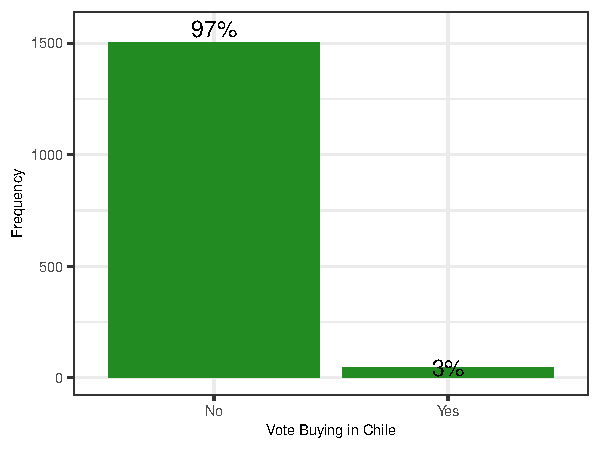
\includegraphics[width=\maxwidth]{figure/client:lapop:plot-1} 

}

\caption{{\bf Frequency and Percentages Vote Buying in Chile}. \\\hspace{\textwidth} {\bf Note}: LAPOP survey data for Chile (2014 wave). Question is \texttt{clien1n}: ``been offered a favor, gift or any other benefit in exchange for their electoral support.'' Only a small proportion have engaged in clientelism. Percentages correspond to the grand total. N = 1,548. 
}\label{fig:client:lapop:plot}
\end{figure}


\end{knitrout}


%
While that is good news, we are rather ignorant about a number of other interesting, and yet, unanswered questions. First and foremost, the approach used by most quantitative scholars focuses exclusively on vote \emph{buying}. That is, the literature usually looks at parties \emph{buying} votes---as the LAPOP survey question conveys---unfortunately, \emph{ignoring} voter's preferences and incentives, particularly, their willingness to sell. This is striking. The clientelist relationship has been clearly described as ``reciprocal'' \parencite[]{Auyero2000}. However, the quantitative study of clientelism has almost ignored this. For instance, the LAPOP question, by exclusively focusing on vote buying, gives the falsely optimistic impression that Chilean voters systematically ``oppose'' vote buying, ``thus'' rarely engaging in clientelism (as \autoref{fig:client:lapop:plot} strongly suggests). 


{\bf My research project seeks to study the supply \underline{and} demand conditions under which clientelist transactions occur, that is, taking into account both parties' \underline{and} voters' incentives}. The project focuses its attention on some conditions such as selling/buying prices, weather voter and party id's match, and levels of electoral uncertainty (i.e. the degree in which the party believes is in risk of losing the election). To study these questions, I seek to implement a series of lab experiments (for which I have already piloted some preliminary designs).

%
\paragraph{Gaps in the Literature} I contend that overlooking the \emph{reciprocal} relationship that exists between vote \emph{buyers} (political parties) and vote \emph{sellers} (voters) {\bf biases} our knowledge about clientelism. In fact, it seems that whether studies focus on vote buying or vote selling depends partly on methodological rather than theoretical decisions. On the one hand, historical and/or ethnographically based contributions describe clientelist transactions from the point of view of voters, focusing on the conditions that make vote selling most likely \parencite{Posada-Carbo:1996aa,Sabato2001,Auyero2000,Szwarcberg2013,Borges2019}. On the other hand, statistical, survey, and/or experimental-based studies mostly explore issues related to vote buying. For example, using a field experiment in Benin, \textcite{Wantchekon2003} stresses the role of incumbency on vote buying. \textcite[227]{Jensen2013a} focus on the impact of ``poverty on vote buying,'' while \textcite[84]{Khemani2015} shows that ``vote buying in poor democracies is associated with lower [public] investments.'' 

Except for several important quantitative studies \parencite{Corstange2012a,Imai2014a,Nichter2014a,Hicken2015,Hicken2018,Auerbach2018,Bahamonde2020a}, the emphasis of statistical studies remains on studying vote buying. In fact, the vast majority of quantitative studies practically overlooks the reciprocal relationships taking place in clientelist transactions (i.e. buyers \emph{and} sellers). Since applied quantitative scholars have systematically neglected the intertwined relationship that exists between vote \emph{buyers} and vote \emph{sellers}, we remain in ignorance about a number of important questions. In fact, the clientelism literature has been quite myopic regarding other aspects other than individual profiles. As \textcite[14]{Carlin2015} correctly point out, ``[e]xisting research [on clientelism] looks almost \emph{exclusively} at individuals' socio-economic and, specially, electoral profiles [and] [y]et our knowledge of who parties target remains incomplete.''\footnote{Emphasis is mine.} My project intends to bridge this gap. 



Finally, another gap in the clientelism literature is that most studies ignore that survey respondents are highly affected by social desirability bias. Social desirability bias happens when survey respondents systematically lie when asked about sensitive, illegal or embarrassing questions (such as selling one's vote). If this bias is not accounted for, our results will inevitably be wrong. To the best of my knowledge, there are no studies about the willingness to sell the vote in Chile that account for social desirability bias. In the study of clientelism the issue of social desirability bias has been addressed in the United States \parencite{Bahamonde2020a} and Latin America \parencite{GonzalezOcantos2014,Gonzalez-Ocantos2012}. Notably, Chile has \emph{not} been studied. 



\section{Objectives, Hypothesis and Research Questions}

\emph{Who do parties target? Who do voters sell their vote to? Under what conditions the supply of votes (voters) and demand for votes (parties) meet?} While these questions might seem obvious, the literature is far from conclusive. \textcite[]{Dixit1996} and \textcite[]{Cox1986} show that parties target their own supporters. Since the ``core constituencies'' are well known individuals to the party machines, they are less likely to defect (that is, take the bribe, and then vote as they wish). However, \textcite[]{Stokes2005} explains that parties target ``moderate opposers.'' She explains that targeting core constituencies is a waste---contradicting \textcite[]{Dixit1996}, and \textcite[]{Cox1986}---and hence, party machines target people whose future support is in doubt. In turn, \textcite[]{Nichter2008} explains that parties target ``unmobilized supporters.'' My research project seeks to contribute to this debate by shedding some light on the following questions.


%Despite these theoretical advances devoted to explain and model the preferences of parties, the literature is silent about the seller's preferences, failing to take the inter-dependent seller-buyer relationship seriously. 



%This project seeks to answer the following unanswered questions: \emph{Would voters still sell their vote to their own party of preference, or would they sell it to the opposing party? Does the selling price vary if selling the vote to the opposing party?} That is, \emph{Do voters set a higher selling price if selling it to the opposing party, while lowering the price if selling to the party they would have supported anyways?} Since the idea is to incorporate both the demand \emph{and} supply side, these questions have a set corresponding mirroring questions. To name a few, \emph{Would parties sell to their own supporters? Moderate opposing voters? Or would they buy opposing votes?} And depending on whose vote is being bought, \emph{Does the price vary?} 



\paragraph{Specific Questions: Economic Experiment} This portion of the project seeks to study the micro dynamics of vote buying and vote selling via an economic experiment (explained in the methods section). My research questions are the following. {\bf For vote buyers}: \emph{Under what conditions do parties buy votes?} \emph{What is the buying price?} \emph{What are the market factors (price, electoral uncertainty, party ID) that foster clientelism?} And {\bf for vote sellers}: \emph{Under what conditions do voters sell the vote?} \emph{What is the selling price?} \emph{Would voters sell their vote to their party of preference, or would they sell it to the opposing party?} \emph{Do voters set a higher selling price if selling to the opposing party, while lowering the price if selling to the party they support?} 


\paragraph{Working Hypotheses: Economic Experiment} (1) The function that determines the probability of vote buying follows a U-inverted shape. {\bf This hypothesis challenges the literature}. As \textcite{Weitz-shapiro} explains it, this relationship is lineal: more competition increases vote buying. I disagree: when the probability of losing/winning the election is high, vote buying is \emph{less} likely. The reason is quite intuitive. When losing the election is the most likely scenario, or when a party feels that the probability of winning the election is high, investments in vote buying represent a waste. However, the probability of clientelism is the highest when it is uncertain whether the party will lose or win the election, that is when there is a 50/50 chance of winning/losing the election. \emph{It is electoral uncertainty, no competition what drives clientelism}. (2) The probability of getting caught decreases the probability of buying and selling votes. (3) All else equal, parties with larger endowments buy \emph{more} votes. {\bf This hypothesis also contradicts the literature}. \textcite[]{Szwarcberg2013} explains that parties with more resources not always buy votes. I disagree. In line with \textcite{Bahamonde2018}, I expect parties to expand their clientele by buying votes from the wealthy too. After bribing the poor, clientelistic parties should move on and engage in expensive clientelism buying votes from the wealthy, if possible. That implies that (4) higher individual incomes do not stop clientelism but increase the selling price of the vote. (5) Selling to the own party lowers the price. However, (6) selling to the opponent party increases the selling price.


\paragraph{Specific Questions: List Experiment} This portion of the project seeks to study the micro dynamics of vote selling via a list experiment (explained in the Methods section). The experiment seeks to understand---in an unbiased way---the conditions under which a sample of Chilean voters are more willing to sell. The research questions for vote sellers are: \emph{Under what conditions do voters sell their vote?} \emph{What is the selling price?}

\paragraph{Working Hypotheses: List Experiment} (1) Chilean voters do sell their votes but at high prices. Since parties cannot afford this strategy, the transaction is not produced---lowering the levels of vote buying (\autoref{fig:client:lapop:plot})---but also putting heavy incentives for parties to connect with their constituencies by offering policy packages rather than clientelism \parencite{Kitschelt2000}. However, (2) Chilean voters do not necessarily value democracy better. That is, while actual levels of clientelism are low/inexistent (\autoref{fig:client:lapop:plot}), that does not imply that their democratic values are high. It only means that the supply and demand of clientelism do not meet. %I believe these methodological improvements untangle any wrong interpretations derived from analyzing \autoref{fig:client:lapop:plot}.


\paragraph{Objectives} Both experiments will provide the necessary data for writing the following papers, which will be circulated at different international conferences, and eventually, published in different international academic WOS-indexed journals. Rest assured, this project is fundamental to build my academic career.

I intend to publish, at least the following papers:


\begin{enumerate}
	\item ``Evaluating Willingness to Sell the Vote in Chile, a List Experiment: Hidden Sellers with High 'Democratic' Values.''
	\item ``An Economic Experiment of Vote Buying and Vote Selling in Chile: the case of price elasticities.''
	\item ``An Economic Experiment of Vote Buying and Vote Selling in Chile: the case of party id's.''
	\item ``An Economic Experiment of Vote Buying and Vote Selling in Chile: the case of competitive elections.''
\end{enumerate}

In addition, this project seeks to achieve the next objectives, all related to scientific divulgation:

\begin{enumerate}
	\item {\bf To advance our knowledge about the micro dynamics of clientelism}. Unlike past research, my project aims to disentangling the---so far ignored---relationship that exists between vote buyers (parties) and vote sellers (citizens). Given that the overall methodology used---yet to be explained and justified in the methods section---is in nature experimental, that will allow me to do so in a non-intrusive way, that is, without generating the social desirability biases associated with the study of clientelism. This methodology, also, will permit modeling the incentives of each player (i.e. voters and parties) in selling/buying votes, as well as modeling the incentives of defecting (i.e. accepting the bribe and then defecting). I do so by modifying (1) the probability of being caught, (2) manipulating the size of the initial endowment for both parties and voters, (3) manipulating the type (i.e. id) of each player---whether parties buy from supporters or opposers. As I explain later, modeling these parameters allows me to emulate (1) the quality of electoral institutions, (2) differences in party/voters endowments, (3) the dual relationship between vote sellers and vote buyers.
	
	\item {\bf To refine our criteria in terms of public policy.} The papers will not only advance our academic knowledge about clientelism in Chile, but also help us in understanding---and importantly too---\emph{diagnosing} the ``democratic health'' of the Chilean electorate. Particularly, the survey experiments will be the firsts of their kind in eliciting \emph{truthful} answers from actual voters about clientelism. The approach is novel. Using a series of statistical techniques which I will explain later, I will be able to predict the individual probabilities of vote selling. This piece of information will be studied along other questions to capture levels of democratic support. What we learn, in turn, is where we, as a society, should put our attention to when it comes to educating our citizens. \emph{What can be rethought in terms of implementing civic courses in elementary school? How can we think about a better and stronger citizenship?} These interesting, and fundamental questions, will be addressed in three public lectures at the \emph{Universidad de O'\ \unskip Higgins}. I consider writing some op-ed pieces regarding this issue too, particularly linking these findings with the social unrest process of 2019.

	\item {\bf To open up the debate, from a regional perspective, but with an international focus.} The questions mentioned above will be addressed by one widely-known international speaker per year, and myself, in a public conference/event held at the \emph{University}, in Rancagua. Along with that, preliminary results of paper 1 and 2 (year 1), paper 3 (year 2), and paper 4 (year 3), will be presented at these events. This will stimulate the public debate among students, faculty, and the whole regional society. Some of these three public events might also include a speaker from the \emph{Instituto de Ciencias de la Educaci\'on}, particularly, as it relates to early learning developments about citizenship and democracy, in elementary and high-school contexts.
\end{enumerate}

\section{Scientific Novelty of the Proposal}


I find that the quantitative literature of clientelism has failed to look at this phenomenon as a \emph{reciprocal} network of relationships, an issue that my research proposal seeks to shed some light on. Thus, my project does fill a number of important gaps in the literature. 


The bulk of the research project is composed by two experiments (both explained in the methods section). Both experiments advance our substantive and methodological knowledge in the study of clientelism. The economic experiment is relevant to the study of clientelism in Chile because it incorporates both sides of the clientelist relationship (vote buyers and vote sellers). In turn, the list experiment effectively prevents social desirability biases. One important aspect of the economic experiment is that it manipulates price elasticities for both buyers and sellers---i.e. willingness to sell, contingent on discrete increments in both selling and buying prices. In addition, the economic experiment accounts for party identification---an unstudied relationship within the experimental study of vote buying/selling. In turn, the list experiment seeks to study willingness to sell the vote, while accounting for social desirability bias. Since the substantive goal of my proposal is to study the consequences of clientelism, addressing issues of democratic representation, and especially, support for democracy, the list experiment is a particularly important component of the project as a whole.


To conclude, another novelty of my research project is that it studies hypothetical behaviors. This is in fact an unexplored avenue of research in the study of clientelism. I believe that studying hypothetical behaviors---such as the willingness to sell---is a valuable exercise. \textcite[131]{Geddes1990} explains the well-known issues of selection bias of studying ``only cases that have achieved the outcome of interest.'' I contend that scholars should explore latent behaviors as well. Hence, if we are interested in understanding the micro dynamics of clientelism---particularly as a supply-and-demand issue---we should incorporate the preferences of both sellers and buyers. Since the focus of this project is on the willingness to sell, I believe that we can also learn from \emph{unrealized} clientelist transactions. Thus, part of the novelty of my proposal relies on the fact that there is only a couple of studies addressing questions of hypothetical vote buying/selling \parencite{GonzalezOcantos2014,Bahamonde2020a}. Notably, neither study focuses on Chile. 


\section{Methodology}


\paragraph{List Experiment} The study of individual preferences depends on truthful answers. However, there might be circumstances under which individuals might not want to answer truthfully due to social pressure. For instance, in avoiding being judged by the interviewer, individuals might not want to reveal that they have done something illegal, like selling one's vote. 

List experiments administer at random two kinds of lists where different sentences are listed. Both lists look exactly the same (say, each one containing the three same items), however the treatment list includes (traditionally) a fourth item, which is the sensitive item related to the socially-condemned behavior. List experiments have been implemented before \parencite{Corstange2008,Redlawsk2010a,Blair2012,Glynn2013,Imai2014a,KiewietDeJonge2015}. Notably, none in Chile in the context of clientelism. 

To illustrate how list experiments work, lets consider an example. Subjects randomly assigned to the control condition read the following:

\pagebreak[5]
\begin{lstlisting}[frame=lrtb]
Now, you will have to type HOW MANY, if any, of the following illegal activities you might engage in, assuming you would not go to jail.

(1) steal an iPod from a large department store
(2) speed on the highway because you're late for work/school
(3) download your favorite music from the internet illegally

Type in HOW MANY (NOT WHICH), if any, of these things you would do.
\end{lstlisting}


In turn, subjects randomly assigned to the treatment condition read the following list:

%\pagebreak[5]
\begin{lstlisting}[frame=lrtb]
Now, you will have to type HOW MANY, if any, of the following illegal activities you might engage in, assuming you would not go to jail.

(1) steal an iPod from a large department store
(2) speed on the highway because you're late for work/school
(3) sell your vote to a candidate
(4) download your favorite music from the internet illegally

Type in HOW MANY (NOT WHICH), if any, of these things you would do.
\end{lstlisting}

Both lists are identical, except that the treatment list includes the sensitive item in the third place. The important aspect that conceals the true answer is that respondents are asked {\bf how many items} in the list they would endorse, {\bf not which ones}. This particular feature helps in learning about individual's preferences in a non-intrusive fashion. For instance, if an experimental subject answers ``2,'' the interviewer will not know whether that number includes the sensitive item. Consequently, if the survey respondent wants to endorse the sensitive item, the answer will be ``masked'' by the other items in the list. This concealment makes this technique suitable to study socially condemned behaviors such as vote buying \parencite{Gonzalez-Ocantos2012,Hicken2018,Corstange2012a,Corstange2008,Blair2012}, drug use \parencite{Druckman2015}, sexual preferences \parencite{Labrie2000}, attitudes towards race \parencite[]{Kuklinski1997b,Redlawsk2010a}, among others.

Given that both lists are assigned at random, the mean number of nonsensitive activities that respondents endorsed should be equal across the two lists. However, if there are any statistically significant differences between the two means (i.e. treatment and control lists), that should be attributed only to the presence of the sensitive item. Finally, if a survey respondent answers ``4,'' that would naturally imply the endorsement of the sensitive item. Luckily, there are statistical techniques that help in identifying possible design issues \parencite{Blair2012}. 




 %\textcite[]{Blair2012} and \textcite[]{Imai2014a}, explain that given that the individual's characteristics (such as income, party identification, and others) answering ``0'' and ``4'' are fully observed, experimental subjects who answer $1$, $2$ and $3$ can be inferred using multivariate techniques. Using these statistical methods allows inferring who answered ``yes'' to the sensitive item, that is, who would be willing to sell the vote. Using this piece of information, a second follow-up experiment will be conducted in the same survey. IPSOS-Chile will be hired to conduct this list experiment. An \emph{Online} panel of 1,000 subjects will be interviewed. The sample will be drawn 50\% from the \emph{Regi\'on Metropolitana}, and the rest, from other regions. The sample will be split into halves by gender.


\paragraph{Economic Experiment} Economic experiments assign roles and initial endowments at random. They also distribute at the end of the experimental sessions actual payments. Notably, payments vary according to the quality of decisions made by experimental subjects \parencite{Morton:2010ly}. 

In my design, the game is played in several rounds of anonymous party-voter pairs. Individuals with the \emph{party} role seek to win the election. They might or might not want to buy votes. However, if they lose the election, they lose actual money from their given endowment. The idea is to study the tipping point at which clientelism becomes a reasonable strategy. Individuals acting the \emph{voter} role, want their parties to be elected. If their party loses, they lose actual money from their given endowment. Voters might or might not want to sell their vote. Similarly, the idea is to study, for instance, the threshold at which poverty fosters vote selling. Hence, there are strong incentives to win the election, buy/sell votes only when necessary and avoid clientelism when the probability of getting caught is high. Thus, economic experiments put heavy incentives for both players to be as strategic as possible. 

Both players are offered the possibility to sell their votes (voters) or buy votes (parties). My design considers the following exogenous manipulations: (1) the probability of losing the election (electoral uncertainty), (2) the probability of being caught (quality of electoral institutions), (3) initial economic endowments (inequality levels, which apply to voters and parties). For instance, party \emph{A}, facing heavy risks of losing the election, might want to engage in vote buying. \emph{Does party A buys votes from voters A, B, or both? Do A voters sell their votes cheaper to party A, when compared to party B? When is defection most likely?} Also, \emph{Do individuals with lower endowments (the ``poor'') sell their vote systematically more than ``wealthy'' individuals?} 

Ultimately, by repeating this procedure a number of times, I will be able to {\bf recreate a market of vote sellers and vote buyers}. {\bf The specific game to be used is a bargaining game in an extensive form} \parencite{Watson:2007fk}. While omitted in this proposal due to space concerns, the model has already been developed and formally identified using standard game theory techniques.


\paragraph{Experimental Sample} Both samples will be collected by survey research companies/research centers. A standard battery of socio-economic and political questions will be included as well in both experiments. For statistical reasons, the sample size should be of about 1,500 individuals.


\clearpage

\newpage
\section{Work Plan, Schedule and Gantt Chart}

\hypertarget{timing}{I will organize this Gantt chart in three years of four trimesters each}.


\begin{gantt}{19}{12}
    \begin{ganttitle}
      \numtitle{1}{1}{3}{4}
    \end{ganttitle}
    \begin{ganttitle}
\numtitle{1}{1}{4}{1}
\numtitle{1}{1}{4}{1}  
\numtitle{1}{1}{4}{1}
    \end{ganttitle}
    \ganttbar[color=blue]{{\tiny Literature review}}{0}{4}
    \ganttbar[color=red]{{\tiny Programming the experiments}}{1}{3}
    \ganttbar[color=red]{{\tiny Experimental Pretesting, design adjustment}}{2}{2}
    \ganttbarcon[color=green]{{\tiny Field experiments}}{4}{3}
    \ganttbar[color=green]{{\tiny Pre-analysis of data}}{4}{3}
    \ganttbar[color=magenta]{{\tiny Analyze all data}}{4}{7}
    

    \ganttbar[color=cyan]{{\tiny Write paper 1 and 2}}{5}{4}
    \ganttcon{5}{8}{6}{9}
    \ganttmilestone[color=cyan]{{\tiny Public Lecture UOH 1 (preliminary results)}}{6}



    \ganttbar[color=cyan]{{\tiny Write paper 3}}{6}{4}
    \ganttcon{6}{10}{7}{11}
    \ganttmilestone[color=cyan]{{\tiny Public Lecture UOH 2 (preliminary results)}}{7}


    \ganttbar[color=cyan]{{\tiny Write paper 4}}{8}{4}
    \ganttcon{8}{12}{9}{13}
    \ganttmilestone[color=cyan]{{\tiny Public Lecture UOH 3 (preliminary results)}}{9}



    \ganttbar[color=orange]{{\tiny Conferences (national, international), public talks}}{1}{11}
    \ganttbar[color=orange]{{\tiny Incorporate feedback from conferences (revisions)}}{6}{6}



    \ganttmilestone[color=cyan]{{\tiny Submit paper 1 and 2 to WOS journal}}{10}
    \ganttcon{9}{8}{10}{16}


    \ganttmilestone[color=cyan]{{\tiny Submit paper 3 to WOS journal}}{11}
    \ganttcon{10}{10}{11}{17}



    \ganttmilestone[color=cyan]{{\tiny Submit paper 4 to WOS journal}}{12}
    \ganttcon{12}{12}{12}{18}

  \end{gantt}






\newpage
\setcounter{page}{1}
\printbibliography

\end{document}




\section{Work in Progress} 

I have been working on this project for some time now. \emph{Fondecyt de Iniciaci\'on 2022} will allow me to move my research agenda forward. In a first paper \parencite[]{Luna2011}, we identified a number of necessary conditions that, when present, boosted the re-election in a number of important \emph{comunas} in the \emph{Regi\'on Metropolitana}. In total, 6 months of field work was done, and more than 100 interviews, as well as participant observation, were conducted. An important variable was campaign spending, which often times had direct relationship with clientelism and vote buying. 

Since then, I have managed to publish two important pieces in my career---both are about clientelism. First, in \textcite{Bahamonde2018} I looked at the question of who political parties ``\emph{target}''---that is, who political parties seek to give money or resources to, in exchange for their electoral support. {\bf This paper is particularly novel because the literature is silent about whether parties target groups or individuals}. I argue that \emph{parties target groups when there are economies of scales of targeting: by targeting one individual, the untargeted voters cultivate some expectations that they might be targeted in the future}. I called this ``{\bf the positive spillovers of clientelism}.'' I used the logic of game theory, particularly, the idea of repeated games. This piece of research has received some awards, and has been presented in a number of conferences, including, Chicago, New York City, among others. 

Second, in \textcite{Bahamonde2020a} I exploit a novel dataset representative for all the United States (N\;=\;1,479). In particular, I designed a list experiment to ask survey respondents if they \emph{would} sell their votes. In nineteenth-century United States politics, vote buying was commonplace. Nowadays, vote buying seems to have declined. Very much like in Chile, the U.S. has very low levels of actual vote buying. However, I discovered that 25\% would sell their vote for a minimum payment of \$418, and that democrats and liberals are more likely to sell, while education or income levels do not seem to impact the likelihood of vote selling. 

\emph{Fondecyt de Iniciaci\'on 2022} will allow me to continue with this research agenda, uncovering hidden and unexplored patterns about vote selling. It will also allow me to contribute to the understanding of Chilean society by identifying factors that increase the probability of individuals and parties to sell and buy votes. These findings are fundamental for understanding any political system that aspires to consolidate.


\section{Available Resources}

%As a junior scholar of the \emph{Instituto de Ciencias Sociales} at the newly opened \emph{Universidad de O'\ \unskip Higgins}, I have the opportunity---but also the \emph{challenge}--of working at a brand new institution. Fortunately, however, there are a number of available resources. 

Since clientelism and inequality represent the core of my research, and as my publications record suggests, part of the available resources I have come from my ongoing work. Publishing both \textcite{Bahamonde2018, Bahamonde2020a} has helped me to connect with other scholars around the globe. This network of collaborators is an available resource that I intend to use when it comes to circulating the designs and papers in order to get feedback. These networks will also help me putting panels together at prestigious international conferences (REPAL, LASA, ACCP, APSA, MPSA, SPSA and WPSA).

Second, \emph{Universidad de O'\ \unskip Higgins} generously granted a small research grant which allowed me to pilot some preliminary experimental designs programmed in \texttt{Python}. Part of this process led me to build a collaboration network with the \emph{Centro de Ciencias Experimentales Sociales} (CESS) which is a partnership between USACH and Oxford University. In fact the design along with the formal models have been already \href{https://fae.usach.cl/fae/index.php?option=com_content&view=article&id=5903:2019-12-06-17-58-10&catid=13:noticias-fae}{presented} at their colloquium. Since the CESS implements economic experiments, I intend to use this ongoing collaboration network to continue with the project described in this proposal. 

It should be noted that the list experiment needs to be implemented in \texttt{Qualtrics}, a software to implement online surveys. \texttt{Qualtrics} is \emph{very} pricey. Fortunately, not only I have already programmed the list experiment in \texttt{Qualtrics} but also keep having access to this expensive software via my doctoral university. I believe I am saving a huge amount of money with this available resource.

In sum, part of my available resources (some software, networks, preliminary experimental designs programmed in \texttt{Python} along with some already collected data) come from my ongoing work. 

In addition, the \emph{University} will provide the essentials (a desk, Internet connection, and some access to academic sources). The experiment will be loaded online, so virtually any computer allows taking the experiment. The \emph{University} will also provide excellent students, from whom I will draw a research assistant, and two undergraduate thesis writers. This will be an important mentoring experience both for me, and my students. Importantly, it is also my goal to mentor and insert my research assistant in the academic world as much as possible. Finally, the \emph{University} will also provide the logistics for all public talks.




% trabajo adelantado con CESS y python.
% pre-testing
% formal models listos
% presentaciones y feedback
% aceptaciones en congresos





